\documentclass{article} 

\documentclass[aspectratio=169,10pt,dvipsnames]{beamer} 
\usepackage{graphicx}
\usepackage{tabularx}
\usepackage{array}
\usepackage[most]{tcolorbox}
\usepackage{mathtools}
\usepackage{stackengine}
\usepackage{algorithmic}
\usepackage{epstopdf}
\usepackage{lipsum}
\usepackage{pifont}
\usepackage{algorithm}
\usepackage{tikz}
\usepackage{animate}
\usetikzlibrary{decorations.pathreplacing}
\usepackage[export]{adjustbox}
\renewcommand{\thealgorithm}{}
\usetikzlibrary{matrix}
\usepackage{natbib} 
\usepackage{bibentry}
\newcommand{\amin}{\mathop{\text{argmin}}}
\newcommand{\forestgreen}{\color{forestgreen}}
\newcommand{\red}{\color{red}}
\newcommand{\blue}{\color{blue}}
\newcommand{\bx}{\boldsymbol{x}}
\newcommand{\blambda}{\boldsymbol{\lambda}}
\newcommand{\by}{\boldsymbol{y}}
\newcommand{\bz}{\boldsymbol{z}}
\newcommand{\bX}{\boldsymbol{X}}
\newcommand{\bY}{\boldsymbol{Y}}
\newcommand{\bZ}{\boldsymbol{Z}}
\newcommand{\bv}{\boldsymbol{v}}
\newcommand{\bu}{\boldsymbol{u}}
\newcommand{\bxi}{\boldsymbol{\xi}}
\newcommand{\bpsi}{\boldsymbol{\psi}}
\newcommand{\bzeta}{\boldsymbol{\zeta}}
\newcommand{\boldsymbolu}{\boldsymbol{\mu}}
\newcommand{\bQ}{\boldsymbol{Q}}
\newcommand{\bS}{\boldsymbol{S}}
\newcommand{\bT}{\boldsymbol{T}}
\newcommand{\bF}{\boldsymbol{F}}
\newcommand{\bG}{\boldsymbol{G}}
\newcommand{\bd}{\boldsymbol{d}}
\newcommand{\bp}{\boldsymbol{p}}
\newcommand{\bff}{\boldsymbol{f}}
\newcommand{\bc}{\boldsymbol{c}}
\newcommand{\bg}{\boldsymbol{g}}
\newcommand{\bA}{\boldsymbol{A}}
\newcommand{\bB}{\boldsymbol{B}}
\newcommand{\bSigma}{\boldsymbol{\Sigma}}
\newcommand{\bC}{\boldsymbol{C}}
\newcommand{\bE}{\boldsymbol{E}}
\newcommand{\bh}{{\boldsymbol{h}}}
\newcommand{\bH}{{\boldsymbol{H}}}
\newcommand{\bJ}{{\boldsymbol{J}}}
\newcommand{\bR}{{\boldsymbol{R}}}
\newcommand{\bn}{\boldsymbol{n}}
\newcommand{\br}{\boldsymbol{r}}
\newcommand{\bl}{\boldsymbol{l}}
\newcommand{\bI}{\boldsymbol{I}}
\newcommand{\bzero}{\boldsymbol{0}}
\newcommand{\st}{\mathop{\text{s.t.}}}
\newcommand{\diag}{\mathop{\text{\normalfont diag}}}
\newcommand{\aminmax}{\mathop{\text{\normalfont argminmax}}}
\newcommand{\interior}{\mathop{\text{\normalfont interior}}}
\newcommand{\ReH}{\mathop{\text{\normalfont Re}}}

\setbeamertemplate{navigation symbols}{}

\newcommand\blfootnotefirst[1]{%
  \begingroup
  \renewcommand\thefootnote{}\footnote{\color{darkgray}\tiny\vspace{-.13in}\hspace{-.32in}#1}%
  \addtocounter{footnote}{-1}%
  \endgroup
}

\newcommand\blfootnote[1]{%
  \begingroup
  \renewcommand\thefootnote{}\footnote{\color{darkgray}\tiny\vspace{-.02in}\hspace{-.32in}#1}%
  \addtocounter{footnote}{-1}%
  \endgroup
}

\newcommand\with[1]{%
  \begingroup
  \renewcommand\thefootnote{}\footnote{\hspace{-.32in}\normalfont Joint Work with #1}%
  \addtocounter{footnote}{-1}%
  \endgroup
}
\renewcommand\footnoterule{}

%% Colors
\definecolor{forestgreen}{rgb}{0.13, 0.55, 0.13}
\definecolor{green2}{rgb}{0, 0.8, 0}
\definecolor{UWGray}{RGB}{90,90,90}
\definecolor{UWRed}{RGB}{38,72,161}
\setbeamerfont{author}{series=\bfseries}
\setbeamerfont{title}{series=\bfseries}
\setbeamerfont{frametitle}{series=\bfseries}
\setbeamerfont{block title}{size={}}
\setbeamercolor{block title}{fg=UWRed}
\newcommand{\green}{\color{green2}}
\newcommand{\UWgray}{\color{UWGray}}
\newcommand{\UWred}{\color{UWRed}}
\usepackage{cmbright}
% \usefonttheme{professionalfonts} % using non standard fonts for beamer
% \usepackage[utf8]{inputenc} 
% \usepackage[T1]{fontenc}
% \usepackage[frenchb]{babel}
% \usepackage{setspace}
\usepackage{color}
\usepackage{listings}
\lstdefinelanguage{Julia}%
{morekeywords={abstract,break,case,catch,const,continue,do,else,elseif,%
end,export,false,for,function,immutable,import,importall,if,in,%
macro,module,otherwise,quote,return,switch,true,try,type,typealias,%
using,while,@threads,@optinode,@variable,@constraint,@NLnodeconstraint,@linkconstraint,@objective,@optiedge},%
sensitive=true,%
alsoother={$},%$
morecomment=[l]\#,%
morecomment=[n]{\#=}{=\#},%
morestring=[s]{"}{"},%
morestring=[m]{'}{'},%
}[keywords,comments,strings]%
\definecolor{codegreen}{rgb}{0,0.6,0}
\definecolor{codegray}{rgb}{0.5,0.5,0.5}
\definecolor{codepurple}{rgb}{0.58,0,0.82}
\definecolor{backcolour}{rgb}{0.95,0.95,0.92}
\lstdefinestyle{mystyle}{
backgroundcolor=\color{backcolour},   
commentstyle=\color{codegreen},
keywordstyle=\color{magenta},
numberstyle=\tiny\color{codegray},
stringstyle=\color{codepurple},
basicstyle=\ttfamily\footnotesize,
breakatwhitespace=false,         
breaklines=true,                 
captionpos=b,                    
keepspaces=true,                 
numbers=left,                    
numbersep=5pt,                  
showspaces=false,                
showstringspaces=false,
showtabs=false,                  
tabsize=2
}
\lstset{%
language         = Julia,
basicstyle       = \ttfamily,
keywordstyle     = \bfseries\color{blue},
stringstyle      = \color{magenta},
commentstyle     = \color{ForestGreen},
showstringspaces = false,
style            = mystyle
}

\usepackage{pgfplots}
\usepackage{tikz}
\usetikzlibrary{calc}
\usetikzlibrary{colorbrewer}
\pgfplotsset{colormap/blackwhite}

\tikzset{%
  add/.style args={#1 and #2}{to path={%
 ($(\tikztostart)!-#1!(\tikztotarget)$)--($(\tikztotarget)!-#2!(\tikztostart)$)%
  \tikztonodes}}
} 

\beamersetrightmargin{0.025\paperwidth}
\beamersetleftmargin{0.025\paperwidth}

\usepackage{animate}


\definecolor{emph}{rgb}{0.2,0.2,0.7}
\setbeamertemplate{footline}[frame number]
\setbeamertemplate{subsection in toc}{\hspace*{2em}{\footnotesize \inserttocsectionnumber.\inserttocsubsectionnumber.~\inserttocsubsection\par}}
\setbeamertemplate{section in toc}{\inserttocsectionnumber.~\inserttocsection\par}
\usepackage{hyperref}

\usepackage{times}
\usepackage{DejaVuSansMono}

\usepackage{enumitem}
\setitemize{label=\usebeamerfont*{itemize item}%
  \usebeamercolor[fg]{itemize item}
  \usebeamertemplate{itemize item}}

\newcommand{\backupbegin}{
   \newcounter{finalframe}
   \setcounter{finalframe}{\value{framenumber}}
}
\newcommand{\backupend}{
   \setcounter{framenumber}{\value{finalframe}}
}
\usetikzlibrary{positioning, fadings, backgrounds}

\usepackage{multirow}
\newcommand{\reference}[1]{%
  \tikz[remember picture,overlay,align=center]{s
    \node[anchor=south west,color=darkgray,font=\tiny,align=left,inner sep=1] at (current page.south west) {#1};
  }%
}
\title{ExaModels and MadNLP: Open-Source Software Infrastructure for Accelerated Nonlinear Optimization on GPUs}
\author{Sungho Shin$^\dag$, Francois Pacaud$^\ddag$, and Mihai Anitescu$^\dag$} 
\date{\small
  $^\dag$Mathematics and Computer Science Division, Argonne National Laboratory\\
  $^\ddag$Centre Automatique et Systèmes, Mines Paris - PSL, Paris, France
}
\begin{document}
\maketitle 

We are pleased to submit our nominations for the COIN-OR cup, highlighting our contributions of ExaModels and MadNLP in the domain of computational infrastructure for operations research, in the particular area of nonlinear optimization. Our open-source software packages represent a significant advance in addressing the challenges of efficiently solving large-scale nonlinear optimziation problems by harnessing the capabilities of modern GPU hardware. In this document, we highlight the key challenges and opportunities we are facing for the development of optimization software in 2023, especially in the context of the advent of accelerated computing. We also explain how ExaModels and MadNLP jointly address the key technical challanges and harness the benefits that modern accelerated computing has to offer. We also highlight several performance improvement we have achieved in terms of solving large-scale, real-world nonolinear optimziation problems. Finally, we conclude by discussing how our development sets the stage for the next-generation nonlinear optimization solver development and opens up new possibilities in various applications.

\paragraph{Challenges and Significance}
The computational landscape of today presents us with immense challenges and potential opportunities, especially with Graphics Processing Units (GPUs) at our disposal. Notably, NVIDIA GPUs have enabled great stride in the scalabiltiy of deep learning and achieved remarkable success in building large-scale AI models. Also, in the public doamin, most of the computational power for the next generation exascale HPC systems, such as Frontier and Aurora, come from GPU accelerators. While the GPUs have enabled great success in different scientific computing areas, such as machine learning and high-fidelity simulations, utilizing GPUs within nonlinear programming (NLP) algorithms has been hindered by challenges like sparse automatic differentiation (AD) and sparse linear solver routines, which do not seamlessly translate to GPU architecture. The key issue is that the conventional sparse AD and matrix factorization algoirthms are built for CPUs, and they heavily rely on the serial computation. 

While GPU computation can trivially accelerate several parts of the optimization process---especially various internal computations within the optimization solver---the sluggish data transfer between host and device memory hampers the ad-hoc implementation of GPU accelerations (Fig. \ref{fig:memory}). To fully leverage the potential offered by modern GPU hardware, it becomes imperative to have a comprehensive computational framework for optimization on GPUs. That is, we need an AD/algebraic modeling framework, sparse linear solvers, and NLP solvers that can operate entirely on the GPU. Specifically, for the best performance, both the problem data and the solver's intermediate computational data must be exclusively resident within the device memory, with the majority of operations executed on the GPU. This necessitates the development of {\it a comprehensive nonlinear optimization solution framework}, which performs all the necessary computations---automatic differentiation, nonlinear optimization, and linear algebra---exclusively on GPUs. ExaModels and MadNLP rise to these challenges, carving out a pathway to fully harness the power of GPUs for operaitons research and nonlinear optimization. 

\begin{figure}[t]
  \centering
  \scalebox{.87}{
  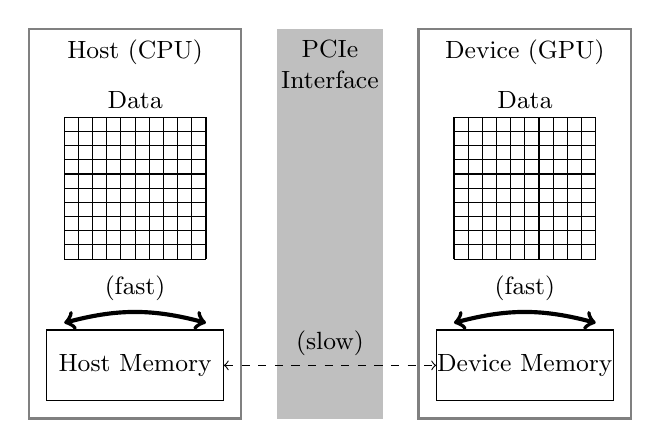
\begin{tikzpicture}[remember picture, scale=.9, font=\small]

    \fill[lightgray] (3.25,-.75) rectangle (4.75,4.75) node[black,midway,align=center,yshift=57.5] {PCIe\\Interface};
    \draw[gray,thick] (-.25,-.75) rectangle (2.75,4.75) node[black,midway,align=center,yshift=62] {Host (CPU)};
    \draw[gray,thick] (5.25,-.75) rectangle (8.25,4.75) node[black,midway,align=center,yshift=62] {Device (GPU)};

    \node[align=center] at (1.25, 3.75) {Data};
    \node[align=center] at (6.75, 3.75) {Data};

    % Host Memory
    \draw (0,-.5) rectangle (2.5,.5) node[midway] {Host Memory};

    % Device Memory
    \draw (5.5,-.5) rectangle (8,.5) node[midway] {Device Memory};


    % Arrow with Dashed Line
    \draw[<->, dashed] (2.5, 0) -- (5.5, 0) node[midway, above, align=center] {(slow)};
    \draw[<->, line width=1.5] (.25, .6) to [in=165, out =15] node[midway, above, align=center] {(fast)}(2.25, .6) ;
    \draw[<->, line width=1.5] (5.75, .6) to [in=165, out =15] node[midway, above, align=center] {(fast)}(7.75, .6) ;

    \def\rows{10}
    \def\cols{10}
    \def\elementwidth{2}
    \foreach \xshift/\yshift in {.25/1.5, 5.75/1.5} {
      % Draw Grid
      \foreach \i in {0,...,\rows} {
        \draw (\xshift, \yshift+\i*\elementwidth/\rows) -- (\xshift+\elementwidth, \yshift+\i*\elementwidth/\rows);
      }
      \foreach \i in {0,...,\cols} {
        \draw (\xshift+\i*\elementwidth/\cols, \yshift) -- (\xshift+\i*\elementwidth/\cols, \yshift+\elementwidth);
      }
    }
  \end{tikzpicture}
  }
  \includegraphics[width=.48\textwidth]{speedup-sol.pdf}
  \label{fig:simd}
  \caption{A schematic of host (CPU) and device (GPU) memory structure (left) and speedup achieved for AC optimal power flow problems (right).}\label{fig:memory}
\end{figure}

\paragraph{Developed Software Tools}
We have developed a comprehesnive nonlinear optimization framework by implementing our algebraic modeling/automatic differentiation tool ExaModels and nonlinear optimization solver MadNLP, while linear algebra computation is currently performed by the external cuSOLVER library. 

{\it ExaModels}: SIMD Abstraction for NLPs: ExaModels pioneers the implementation of a groundbreaking single-instruction, multiple-data (SIMD) abstraction for NLPs. This revolutionary approach unlocks the potential for efficient parallel automatic differentiation on GPUs. The essence of this innovation lies in preserving the parallelizable structure within model equations, transforming derivative evaluations into streamlined operations. By enabling efficient computation of derivatives on GPUs, ExaModels offers an exceptional performance boost for power systems analysis.

The optimization models are most of the times implemented by the researchers and practitioners who do not necessarily understand the operations 
ExaModels provides a new platform for scalable nonlinear optimization. Our numerical results suggest that the conventional algebraic modeling systems are limited in terms of efficiently computing the derivates of the model equations (Table \ref{tab:num}), and it does not allow performing the operations on GPUs (Table \ref{tbl:portabiltiy}). ExaModels provide a framework that allows the user to conveniently inform the AD backend the parallelizable structure. Writing the models in this way will enable the GPU compatibility 

{\it MadNLP}: Condensed-Space IPM with Inequality Relaxation: MadNLP introduces an equally transformative approach through its condensed-space interior-point method (IPM) with an inequality relaxation strategy. This strategy deftly overcomes the challenges posed by sparse matrix factorization on GPUs. The relaxation of equality constraints and condensation of the Karush-Kuhn-Tucker (KKT) system establishes positive definiteness, paving the way for the utilization of highly efficient linear solvers. MadNLP thus unveils a remarkable solution to traditionally intractable problems in GPU-based optimization.

While MadNLP has started as a port of Ipopt on Julia Language, now marking as the fourth year since its initial development, MadNLP has become a lot more versatile solver than the previously developed nonlinear optimization solvers. The key features include (1) being able to solve dense optimzation problems, (2) ability to handle different forms of KKT systems, (3) being able to handle diverse array data types (most notably, device arrays), and (4) exploit various Hessian approximation strategies (BFGS variants and limited-memory BFGS methods).

\paragraph{Performance Highlights}

The significance of these contributions is not merely theoretical. Empirical results speak volumes about the impact of ExaModels and MadNLP. When applied to AC OPF problems, the performance enhancements achieved are nothing short of extraordinary. The GPU-based solutions attain speedups of over 20 times compared to CPU-based counterparts, showcasing the profound potential of these software packages in power systems analysis. Their prowess surpasses even established tools interfaced with CPUs, marking a paradigm shift in computational efficiency.

\cite{shin2023accelerating}
 
\begin{table}[t]
  \begin{center}
    \begin{tabular}{|l|c|c|ccc|ccc|}
  \hline
  \multirow{3}{*}{\textbf{Case}}
  & \multirow{3}{*}{\# vars}
  & \multirow{3}{*}{\# cons}
  & \multicolumn{3}{c|}{\textbf{MadNLP+ExaModels+cuSOLVER}}
  & \multicolumn{3}{c|}{\textbf{Ipopt+AMPL+Ma27}}
  \\
  & & &\multicolumn{3}{c|}{\textbf{(GPU$^*$)}} &\multicolumn{3}{c|}{\textbf{(CPU$^{**}$)}}
  \\
  \cline{4-9}
  & & 
  & \quad \# iter \quad& \quad AD$^\dag$  \quad&  \quad total$^\dag$ \quad
    & \quad \# iter \quad& \quad AD$^\dag$  \quad&  \quad total$^\dag$ \quad
  \\
  \hline
  10480\_goc 
  &  96.8k
  & 150.9k
  & 70 
  &  0.13
  & 14.26
    & 64 
      & 16.93
                                               & 38.04
  \\

  13659\_pegase 
  & 117.4k
  & 170.6k
  & 63 
  &  0.12
  &  7.15
    & 64 
      & 19.70
                                               & 35.66
  \\

  19402\_goc 
  & 179.6k
  & 281.7k
  & 79 
  &  0.17
  & 23.28
    & 70 
      & 36.50
                                               & 95.34
  \\

  24464\_goc 
  & 203.4k
  & 313.6k
  & 63 
  &  0.11
  & 70.63
    & 58 
      & 33.50
                                               & 70.15
  \\

  30000\_goc 
  & 208.6k
  & 307.8k
  & 162 
  &  0.33
  & 22.05
    & 180 
      & 101.98
                                               & 249.81
  \\
    \hline  
\end{tabular}
    \vspace{-1em}
    \footnotesize
    $^\dag$Wall time (sec) measured by Julia. $^\ddag$CPU time (sec) reported by Ipopt.  \caption{Numerical Performance of ExaModels and MadNLP}
  \end{center}
  \label{tab:num}
\end{table}

\paragraph{Portability}

While NVIDIA seems to be most capable in computing power and mature in terms of the implementation of the low-level operations (especially, the CUDA libraries), we aim to support all the other alternative architectures. This is because quite a few next-generaiton exascale high-performance computing architectures will be based on AMD and Intel accelerator devices. Also, as an open-source software, we aim to be the most generic software tool, not the most efficient one. By supporting diverse platforms, we hope to spark the attention of the chip makers in the operations research area and encourage better support for the software infrastructure for implmenting operations research software. 

Table \ref{tbl:portabiltiy} summarizes the current state of the portability of our tools and other existing open-source software tools. Notably, ExaModels.jl already support all major architectures, whereas MadNLP.jl only support NVIDIA GPUs. Nonetheless, we have clear path forward in supporting all the major accelerator architectures, including NVIDIA, AMD, and Intel GPUs, while Apple GPUs are somewhat limited due to their inability to perform double precision operations. This is due to the fact that all of our GPU kernels are implemented via KernelAbstractions.jl, a julia package enabling portable implementation of GPU kernels. In this way, the GPU kernels for diverse accelerator architectures can be run based on a sam source code. Using this strategy, recently ExaModels.jl has demonstrated its capabiltiy to run on 4 different accelerator architectures (multi-thread CPUs and NVIDIA, AMD, and Intel GPUs). In the coming years, we plan to exand MadNLP's support for various accelerator architectures.

However, at the same time, it is absolutely crucial to have efficient and reliable, and preferrably also portable sparse linear sovler routines. Currently, we rely on CUSOLVER library for solving the linear systems. While vendor-implmented libraries are expected to have the best performance via high level of optimization, it would be beneficial for the community to have the open-source portable linear solvers. By showcasing the capability of solving high-stake nonlinear optimziation problems on GPUs, we can attract the attention of the numerical linear algebra community so that we can encourage the development of capable open-source sparse linear solvers. 
1
\begin{table}[t]
  \begin{center}
    \scalebox{0.72}{
      \begin{tabular}{|c|c|cccccc|}
        \hline
        &&CPU (single) &CPU (multi)& NVIDIA & AMD & Intel& Apple\\
        \hline
        \multirow{3}{*}{Modeling Platforms}& {\bf AMPL}& \cmark& \xmark& \xmark& \xmark& \xmark& \xmark\\
        &{\bf JuMP}& \xmark& \cmark& \xmark& \xmark& \xmark& \xmark\\
        &{\bf ExaModels}& \cmark& \cmark& \cmark& \cmark& \cmark& \xmark\\ 
        \hline
        \multirow{2}{*}{Solvers} & {\bf Ipopt}& \cmark& \xmark& \xmark& \xmark& \xmark& \xmark\\
        & {\bf MadNLP} & \cmark& \xmark& \cmark& \xmark& \xmark& \xmark\\
        \hline
      \end{tabular}
    }
  \end{center}
  \caption{The current status on the portability of the nonlinear optimization frameworks.}
  \label{tbl:portabiltiy}
\end{table}

\paragraph{Impacts in Various Applications}

{\it Energy Infrastructures.} The resillience We have recently showcased the capability of MadNLP with multiple GPUs for solving extremely-large scale security-constrained AC OPF problems.

{\it 1}

{\it Machine Learning Surrogate Models.}

\paragraph{Closing Remarks}
ExaModels and MadNLP embody the spirit of innovation and progress that the COIN-OR cup seeks to recognize. By addressing critical challenges and introducing transformative strategies, these packages extend the frontiers of computational infrastructure for operations research. We are confident that their exceptional contributions will resonate within the operations research community and beyond, redefining the future of power systems analysis and optimization. It is with great enthusiasm that we nominate ExaModels and MadNLP for the COIN-OR cup, recognizing their exceptional impact on the field.

\bibliography{main}

\end{document}